\chapter{Iteration 1: Design and Implementation}

\section{Proof of Concept (POC-Lite) Evolution}
The proposal POC-Lite conceptualized a neighbourhood mobile application with item listings, community chat, and simple location filtering. In Iteration 1, this concept evolved into a production-grade vertical slice architecture. Peripheral non-essential features (e.g., social feed walls, vendor storefronts, unconstrained chatbots) were intentionally stripped out to focus entirely on the complex computing core: \textit{an event-sourced borrowing lifecycle backed by an empirical Bayesian trust engine and cryptographic auditability.}

\section{Computational Core: The Assurance Engine}
The computational core is engineered as a multi-stage pipeline:
\begin{enumerate}
    \item \textbf{Outcome Extraction:} Queries historical transaction events to derive verified objective metrics (on-time return, condition agreement, dispute-free closure).
    \item \textbf{Bayesian Direct Estimation:} Evaluates the borrower's empirical track record using a recency-weighted Beta posterior distribution with analytical 90\% credible intervals and effective sample size calculation.
    \item \textbf{Contextual Similarity Weighting:} Modulates historical observation weights based on the similarity between past transactions and the currently requested loan.
    \item \textbf{Bounded $k$-Hop Indirect Traversal:} Discovers multi-hop trust paths between lender and borrower across the community graph, decaying strength exponentially with topological distance.
    \item \textbf{Context-Aware Decision Policy (Algorithm 4):} Maps direct evidence, indirect paths, item value tier, and locality into decision tiers (Rules R1--R9) and compiles human-readable explanations.
\end{enumerate}

\section{Slice A Completed Implementation}
Slice A establishes the end-to-end transaction lifecycle, implemented across the following components:
\begin{itemize}
    \item \textbf{Domain Aggregate (\texttt{BorrowingTransaction}):} Implements the core entity that applies state events in sequential order. Reconstructs state via \texttt{replay(events)} and enforces transition validity against \texttt{TransitionTable}.
    \item \textbf{Append-Only Event Store (\texttt{PostgresEventStore}):} Appends immutable events to the \texttt{lifecycle\_events} table. A PostgreSQL trigger prevents updates or deletions. Each event records stream ID, sequence number, event type, timestamp, payload, and a SHA-256 hash chaining back to the predecessor event.
    \item \textbf{Application Service (\texttt{BorrowingService}):} Coordinates loan creation, validates temporal bounds, invokes locality verification, generates initial assessment records, and coordinates accept, decline, handover, and return operations.
    \item \textbf{RESTful API (\texttt{routes.py}):} Implements versioned endpoints under \texttt{/api/v1} with JWT authentication and argon2 password hashing. Endpoints include \texttt{/auth/login}, \texttt{/items}, \texttt{/requests}, \texttt{/requests/\{id\}/accept}, \texttt{/requests/\{id\}/handover}, and \texttt{/requests/\{id\}/return}.
    \item \textbf{Mobile/Web Interface (Expo Router):} Delivers a responsive client implemented in React Native and TypeScript, featuring item browsing, loan request submission, and state-aware action bars.
\end{itemize}

\section{Slice B Completed Implementation}
Slice B implements the full mathematical trust pipeline, replacing the initial Slice A placeholder:

\subsection{B1: Outcome Extraction}
Implemented in \texttt{backend/app/domain/assurance/estimation/outcomes.py}. Pure domain rules (Team Decision D11) map closed loan events into verified borrower and lender outcomes:
\begin{itemize}
    \item Borrower metrics: \texttt{ON\_TIME\_RETURN}, \texttt{CONDITION\_AGREED}, \texttt{DISPUTE\_FREE}.
    \item Lender metrics: \texttt{CONDITION\_AGREED} (item accurately described), \texttt{DISPUTE\_FREE}.
    \item Database integration: \texttt{PostgresOutcomeWriter} synchronizes outcomes incrementally from \texttt{v\_pending\_outcomes} upon loan completion.
\end{itemize}

\subsection{B2: Bayesian Beta Posterior and Contextual Similarity}
Implemented in \texttt{posterior.py} and \texttt{similarity.py}. The posterior updates prior $\text{Beta}(\alpha_0, \beta_0) = \text{Beta}(1, 1)$ with recency-weighted successes $s_w$ and failures $f_w$:
\begin{equation}
    w_i = \exp\left(-\frac{\Delta t_i \ln 2}{T_{\text{half}}}\right), \quad s_w = \sum_{i \in S} w_i \cdot \text{sim}_i, \quad f_w = \sum_{j \in F} w_j \cdot \text{sim}_j
\end{equation}
Similarity weighting (Team Decision D17) calculates multidimensional closeness:
\begin{equation}
    \text{sim} = 0.4 \times \text{sim}_{\text{value}} + 0.4 \times \text{sim}_{\text{category}} + 0.2 \times \text{sim}_{\text{duration}}
\end{equation}
The analytical 90\% credible interval $[\theta_{\text{lower}}, \theta_{\text{upper}}]$ is derived from the Beta cumulative distribution function.

\subsection{B3: Bounded $k$-Hop Graph Traversal}
Implemented in \texttt{backend/app/domain/assurance/indirect/khop.py}. Searches the \texttt{trust\_edges} projection for paths between lender $u$ and borrower $v$ up to $k = 3$ hops. Path strength decays by factor $\gamma^h$ ($\gamma = 0.7$). To prevent sybil path inflation, at most one path is admitted per initial neighbour, and multi-path aggregation applies the noisy-OR model capped at $\rho_{\text{sup}} = 0.30$.

\subsection{B4: Decision Policy and Structured Explanations}
Implemented in \texttt{backend/app/domain/assurance/policy/}. Algorithm 4 evaluates the computed parameters against versioned configuration thresholds (\texttt{engine.json} v1.2.0):
\begin{itemize}
    \item \textbf{Rule R1 (Sufficient Evidence):} $E[\theta] \ge 0.75$, $\theta_{\text{lower}} \ge 0.60$, $n_{\text{eff}} \ge 3.0$. Recommends standard handover.
    \item \textbf{Rule R2 (Sufficient with Safeguards):} High-value item tier or moderate variance. Recommends daylight public handover and identity check.
    \item \textbf{Rule R6 (Sparse / Cold Start):} $n_{\text{eff}} < 3.0$, zero adverse signals. Categorized as \texttt{INSUFFICIENT\_EVIDENCE} with precautionary safeguards (no punitive action).
    \item \textbf{Rule R9 (Elevated Risk / Hold):} Adverse direct outcomes or unresolved conflicts. Recommends manual review by community moderator.
\end{itemize}

\subsection{B5: Synthetic Scenario Suite and Verification}
Suite 11 in \texttt{backend/tests/scenarios/} validates the engine across 20 synthetic scenario fixtures and realistic community datasets (\texttt{neighborhood-sim}). Tests verify deterministic convergence, interval bounds, and decision consistency.

\subsection{B6: Lender Evidence Presentation Screen}
Implemented in \texttt{frontend/src/components/request/AssurancePanel.tsx}. Presents a three-layer progressive disclosure dashboard:
\begin{enumerate}
    \item \textbf{Layer 1 (Status \& Safeguards):} Clear plain-language recommendation and required physical precautions.
    \item \textbf{Layer 2 (Evidence Breakdown):} Verified past loans count, effective sample weight, and community path connections (display names only; no private IDs).
    \item \textbf{Layer 3 (Technical Details):} Numerical credible intervals, half-life parameters, and \texttt{config\_version} for audit review.
\end{enumerate}

\begin{figure}[htbp]
\centering
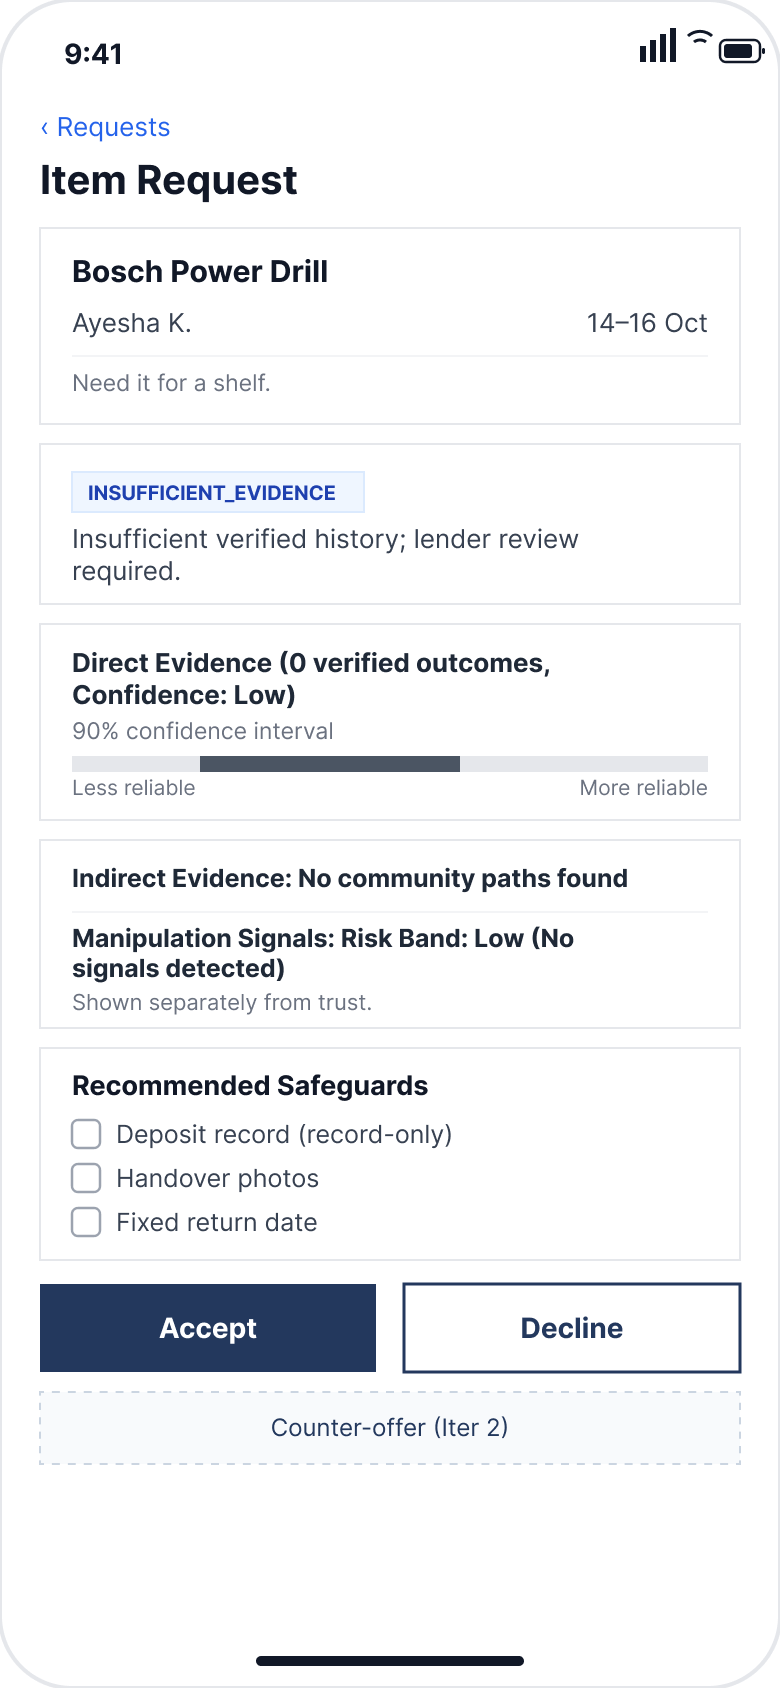
\includegraphics[width=0.45\textwidth]{figures/W1_Lender_Request_Assurance_1.png}
\hfill
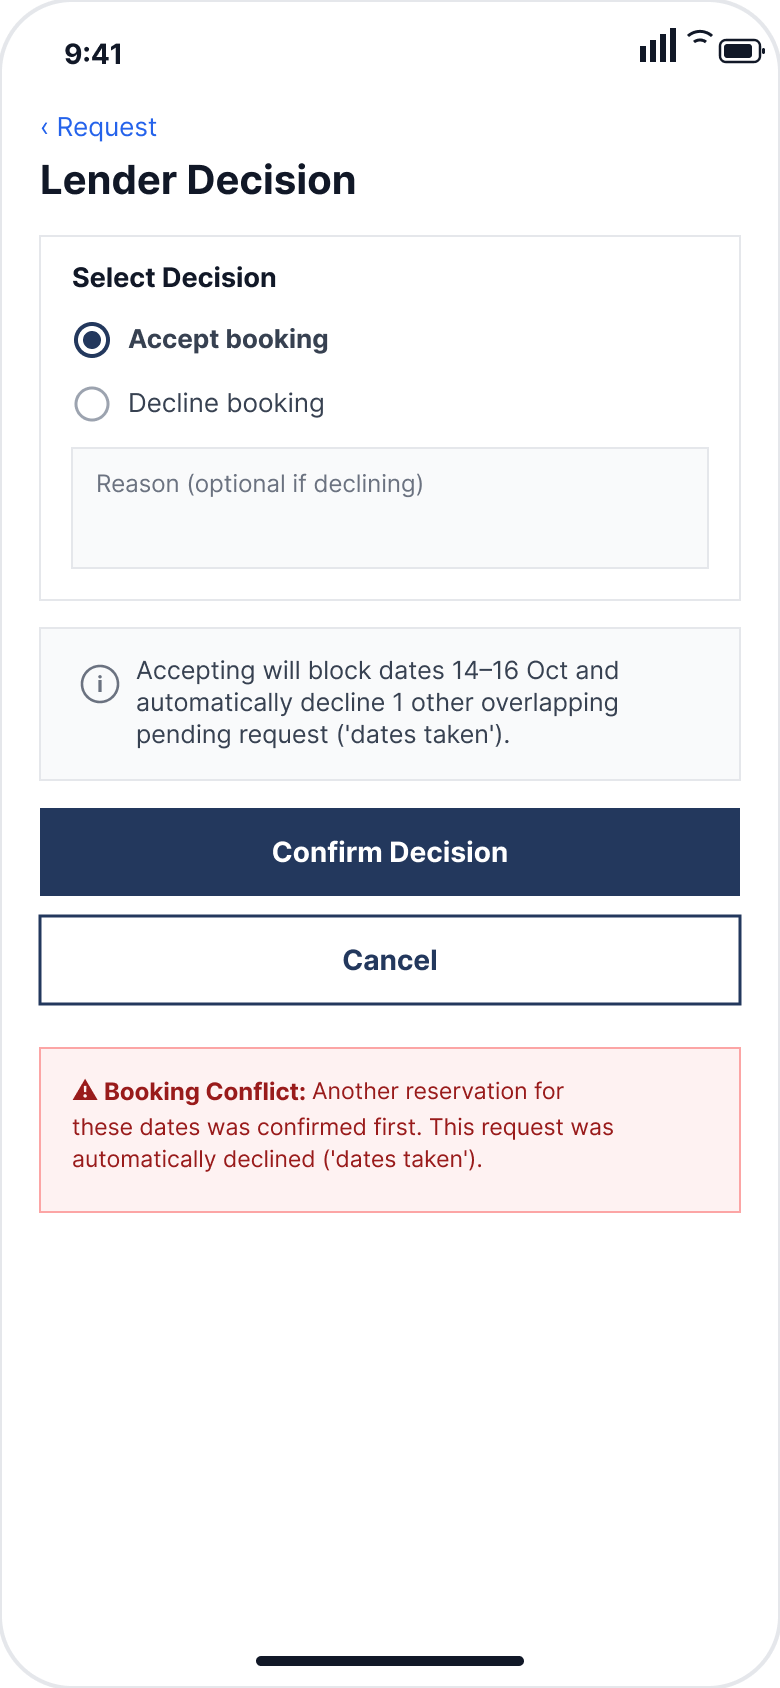
\includegraphics[width=0.45\textwidth]{figures/W2_Lender_Decision_Conflict_1.png}
\caption{UI Implementation: (Left) Lender Request Assurance Dashboard (W1); (Right) Decision Conflict and Escalation Screen (W2)}
\label{fig:lender_wireframes}
\end{figure}

\section{Slice C Implementation and Verification}
Slice C encompasses adversarial manipulation detection and the human moderation loop, fully implemented and verified in the codebase:
\begin{itemize}
    \item \textbf{Manipulation Detection:} Algorithmic detection of rapid review bursts, pairwise reciprocal collusion (S1), review text similarity via character 3-gram TF-IDF (S4), weighted combination with risk bands and corroboration capping (ADR-0007), and retaliatory rating detection that sets contested feedback aside without corrupting trust baselines. Verified across TC-30, TC-38, TC-43, TC-44, and synthetic scenarios ES-04/ES-05.
    \item \textbf{Dispute Resolution Workflow \& Moderation App:} Filing contested return reports (UC-B12, FR-B-16/17), immediate state freezing while DISPUTED (ADR-0004), compilation of tamper-evident audit packets (UC-D6), moderator triage queue (W6), case adjudication (W7), and dispute resolution with safeguards (UC-I4, FR-T-11, ADR-0003). Verified across TC-50--57 and mobile screen tests TC-105--107.
\end{itemize}

\section{Technologies and Tools Used}
\begin{table}[htbp]
\centering
\caption{Implementation Technology Stack and Versioning}
\label{tab:tech_stack}
\small
\begin{tabularx}{\textwidth}{l l p{6.5cm}}
\toprule
\textbf{Subsystem} & \textbf{Technology} & \textbf{Architectural Role / Version} \\
\midrule
Language & Python 3.12 & Backend runtime environment \\
Web Framework & FastAPI 0.115+ & High-performance asynchronous REST API \\
ORM \& Migrations & SQLAlchemy 2.0 / Alembic & Synchronous database access and migration versioning \\
Database & PostgreSQL 16 & Relational persistence, exclusion constraints, triggers \\
Database Driver & psycopg 3 (binary) & High-efficiency PostgreSQL communication \\
Security & argon2-cffi / PyJWT & Cryptographic password hashing and JWT token management \\
Mathematics & NumPy / SciPy & Beta distribution functions and CDF intervals \\
Mobile/Web Frontend & React Native (Expo SDK 52) & Cross-platform Android and web presentation client \\
Typing \& Contracts & TypeScript / openapi-typescript & End-to-end static contract synchronization \\
Testing & pytest, Hypothesis, Jest & Multi-tiered unit, property, and integration test runners \\
Containerization & Docker & Container packaging and local reproducibility \\
Deployment & Render \& Neon & Managed API hosting, static web hosting, and cloud PostgreSQL \\
\bottomrule
\end{tabularx}
\end{table}

\section{Key Technical Decisions and Trade-offs}
\begin{itemize}
    \item \textbf{Synchronous vs. Asynchronous Database Access:} SQLAlchemy 2.0 sync engine with psycopg 3 was selected over asyncpg to guarantee deterministic transaction boundaries and simplify thread-safe event-store sequence checks.
    \item \textbf{Decoupled Configuration:} All engine parameters reside in \texttt{engine.json}. Hardcoding mathematical thresholds in Python code is strictly forbidden.
    \item \textbf{Synthetic Evaluation Rigor:} To prevent academic dishonesty, all evaluation datasets are explicitly derived and labeled as synthetic. No fabricated empirical claims are permitted.
\end{itemize}
